\section{Realios mašinos projektas}

\subsection{Techninės įrangos komponentai}

\begin{figure}[H]
  \begin{center}
    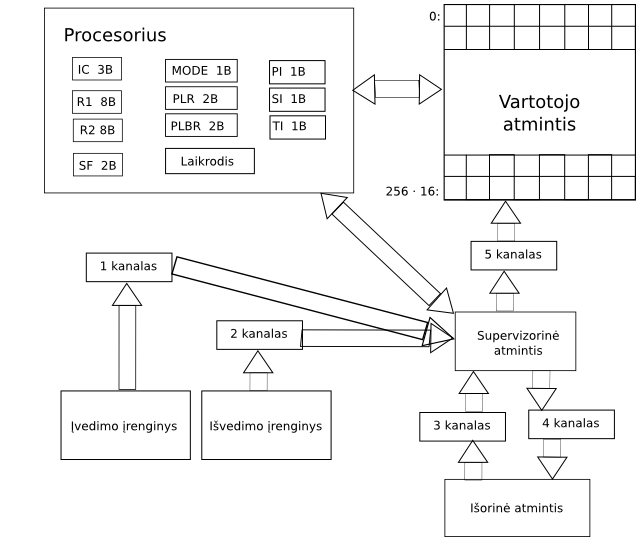
\includegraphics[width=1.0\linewidth]{rm.png}
  \end{center}
  \caption{Realios mašinos architektūra.}
  \label{fig:rm}
\end{figure}

\begin{description}
  \item[Procesorius] Registrų aprašymas:
    \begin{description}
      \item[IC] 3 baitų registras. Skirtas nurodyti vykdomos virtualios
        mašinos komandos adresą atmintyje.
      \item[R1] 8 baitų bendro naudojimo registras.
      \item[R2] 8 baitų bendro naudojimo registras.
      \item[PLR] 2 baitų registras. Skirtas nurodyti puslapių lentelės 
        bloko adresą.
      \item[PLBR] 2 baitų registras. Skirtas nurodyti puslapių lentelės
        pirmojo baito vietą \verb|PLR| bloke.
      \item[MODE] 1 baito registras, kurio reikšmė nusako procesoriaus
        darbo rėžimą (vartotojas, supervizorius).
      \item[SF] 2 baitų registras, skirtas saugoti aritmetinių operacijų 
        loginių (tiesa „1“ arba klaidinga „0“) reikšmių sekai.
      \item[PI] 1 baito registras programiniams pertraukimams fiksuoti.
      \item[SI] 1 baito registras supervizoriniams pertraukimams fiksuoti.
      \item[TI] 1 baito registras taimerio pertraukimams fiksuoti.
      \item[Laikrodis] procesoriaus laiko matavimo įrenginys.
    \end{description}
  \item[Vartotojo atmintis] atmintis skirta virtualių mašinų atmintims bei 
    puslapių lentelėms laikyti. Jos dydis 256 blokai po 16 žodžių, kur
    žodžio ilgis yra 8 baitai. Atmintis numeruojama nuo 0. 

    Pirmieji 16 blokų yra rezervuoti puslapiavimo mechanizmui. Registru
    \verb|PLR| nurodoma, kuriame bloke yra saugoma lentelė, o registru
    \verb|PLBR| nurodoma, kuriuo baitu bloke prasideda puslapių lentelė.
    Atminties baite, kurio pozicija yra $PLR \cdot 16 + PLBR$ ir po jo 
    esančiame baite yra saugoma, kiek blokų užima kodo segmentas 
    (pažymėkime $C (1 \leq C)$). Kitoje baitų poroje nurodyta kiek blokų 
    užima duomenų segmentas (pažymėkime $D (0 \leq D)$). Toliau yra 
    $C$ baitų porų, kuriose nurodyta kokie blokai atitinka kodo puslapius.
    Analogiškai, po jų yra $D$ baitų porų, kurie nurodo kokie blokai 
    atitinka, kuriuos duomenų puslapius.

    Kiti 240 blokų yra skirti virtualių mašinų duomenims.
  \item[Supervizorinė atmintis] jos dydis 16 blokų.
  \item[Išorinė atmintis] kietasis diskas.
  \item[Duomenų perdavimo kanalai] yra 4. 
    \begin{description}
      \item[1 kanalu] perduodami duomenys iš įvedimo įrenginio į 
        supervizorinę atmintį.
      \item[2 kanalu] perduodami duomenys iš supervizorinės atminties
        į išvedimo įrenginį.
      \item[3 kanalu] perduodami duomenys iš kietojo disko į supervizorinę
        atmintį.
      \item[4 kanalu] perduodami duomenys iš supervizorinės atminties į 
        kietąjį diską.
      \item[5 kanalu] perduodami duomenys iš supervizorinės atminties į 
        vartotojo atmintį.
    \end{description}
  \item[Įvedimo ir išvedimo įrenginiai] klaviatūra ir ekranas.
\end{description}

Komandų argumentai nurodyti 16-ainiais skaičiais.

Programuotojas turi nurodyti kokio dydžio duomenų segmentą 
išskirti programai.

\section{Virtualios mašinos aprašas}

\subsection{Virtualios mašinos samprata}

Virtuali mašina - tai tarsi realios mašinos kopija. Virtualioje mašinoje
surenkame mums reikalingus komponentus, tokius kaip procesorius,
atmintis, įvedimo/išvedimo įrenginiai, suteikiame jiems paprastesnę
vartotojo sąsają. Tuo pačiu palengvinamas programavimo procesas,
nes sudėtingas ar vartotojui nepatogias sąsajas virtualioje mašinoje yra 
aprašomos supaprastintai. Virtuali mašina realizuoja realios mašinos
komandas paprastesniu, lengviau suprantamu būdu. Taip pat virtuali mašina
pateikia supaprastintą atminties valdymą. Visa tai leidžia pasiekti realią
ir virtualios mašinos mašininiu kodu parašytą programą sėkmingai įvykdyti
realioje mašinoje. 
